
\section{Color Palette Estimation}
\label{sec:cpe}

In diesem Abschnitt wird eine Algorithmus zur Lösung des Teilproblems $f_{CPE}$ ermittelt. Dies bedeutet die Festlegung eines Verfahrens zur Abbildung $I \to P$, wobei $P = (c_1, ..., c_n)$ die Bildvorlage $I$ mit einer minimalen Menge von Farben repräsentiert. \autoref{sec:cpe-ueberblick} bietet einen Überblick über vorhandene Algorithmen zur CPE. Im Anschluss wird  eine konkrete Methoden ausgewählt und in \autoref{sec:cpe_acopa} erläutert.

\subsection{Überblick}
\label{sec:cpe-ueberblick}

Grundlegend sind zwei Ansätze zur CPE zu unterscheiden:
\begin{enumerate}
    \item \textbf{Histogramm-basiert}: Algorithmen, die von der räumliche Anordnung der Farben im Bild abstrahieren und $P$ auf Grundlage der globalen Farbinformation bilden, d.h. des Histogramms. Da der Definitionsbereich eines Histogramm eine Teilmenge des Farbraums bildet, entspricht dieser Fall der unüberwachten Klassifizierung des Farbraums. Die Umsetzung erfolgt überwiegend durch Clustering-Verfahren, die Gruppen ähnlicher Farben im Bild identifizieren.
    \item \textbf{Segmentierungs-basiert}: Algorithmen, die die räumliche Anordnung der Farben im Bild berücksichtigen. Durch eine Segmentierung des Bildes werden zusammenhängende Komponenten identifiziert, für welche im Folgenden repräsentative Farben ermittelt werden. Die menschlichen Wahrnehmungseigenschaften auf Komponentenebene werden auf diese Weise besser berücksichtigt, gleichzeitig wird durch die zusätzliche Betrachtung der Positionsinformation eine weitere Ebene der Komplexität eingeführt \citep{colorthemes}.
\end{enumerate}

\citet{image-based-schemes} kritisieren an den segmentierungs-basierten Verfahren, dass sie von einer akkuraten Bildsegmentierung abhängen, welche nicht für jede Bildstruktur gewährleistet ist (z.B. in stark texturierten Bereichen). Aus diesem Grund wird für die weitere Diskussion der Fokus auf die histogramm-basierten Verfahren gelegt.

\citet{categorization} treffen eine Kategorisierung der histogramm-basierten Verfahren in \emph{hierarchisch} und \emph{iterativ}. Hierarchische Verfahren starten vor dem Erreichen der (fest zu wählenden) Farbanzahl $n$ mit mehr (\emph{bottom-up}) bzw. weniger (\emph{top-down}) Clustern. Die Aufspaltung bzw. Vereinigung von Clustern basiert auf der statistischen Analyse der Verteilung der Bildfarben im Farbraum. Hierzu zählen unter anderem die in der Vergangenheit populären top-down Raumunterteilungs-Algorithmen wie z.B. Mediancut \citep{mediancut} oder Octree \citep{octree}, welche den Farbraum sukzessiv in disjunkte Teilräume zerlegen und dabei den Clustern eine Würfelform unterstellen. Hierin begründet ebenfalls die Kritik an diesen Verfahren. Ergebnis der Verarbeitung ist ein Dendogram, dessen Blätter die Farben der Farbpalette repräsentieren.

Ein Schnitt des Dendograms entspricht einer Partitionierung des Raums, was dem Ergebnis der iterative Verfahren entspricht.  Sie starten bereits mit der erforderlichen Anzahl Clustern $n$ und optimieren deren Position iterativ entsprechend einer Zielfunktion. Ein Beispiel ist die Minimierung des quadratischen Fehler, wie z.B. bei K-Means \citep{kmeans, kmeanshsi} oder Fuzzy C-Means \citep{fuccycmeans}. Andere Verfahren analysieren das Histogramm auf dichte bzw. weniger dichte Regionen, wie z.B. der Mean-Shift Algorithmus \citep{meanshift}. Die Kritik der iterativen Verfahren begründet sich in deren Abhängigkeit von den Startbedingungen \citep{acopa}.

Für eine detailliertere Vorstellung von Algorithmen zur CPE verweist der Autor auf \citet{categorization2}.

\begin{figure}[h]
\centering
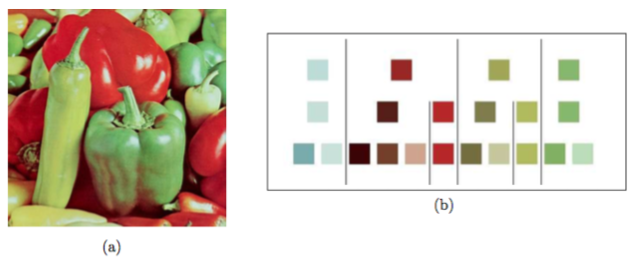
\includegraphics[width=0.48\textwidth]{img/peppers.png}
\caption{CPE Ergebnis von ACoPa. (a) Originalbild "Peppers". (b) Hierarchische Farbpalette. Die oberste Ebene identifiziert die wesentlichen Farbtöne. Ebene 2 bildet Sättigungsstufen. Ebene 3 schlüsselt das Ergebnis weiterhin in Helligkeitsstufen auf und zeigt die finalen Farben. (Quelle: \citep{acopa})}
\label{fig:peppers}
\end{figure}

\citet{acopa} kritisieren an den bisherigen Algorithmen, dass die Anzahl $n$ gesuchter Farben zuvor bekannt sein muss und dass Farben kleiner Bilddetails im Sinne der Definition aus \ref{sec:bildvorlagen} nur unzureichend repräsentiert werden. Dies begründet sich in der Tatsache, dass die bisherigen Verfahren eine Raumunterteilung vornehmen, ohne die Spezifika von Farbräumen zu beachten.

Demgegenüber stellen \citet{acopa} und \citet{image-based-schemes} zwei ähnliche, hierarchische Verfahren vor, die sich die Verwandtschaft der menschlichen Farbbeschreibung mit der Farbkodierung in Farbräumen mit Polarkoordinaten-Repräsentation zu Nutze machen. Sie basieren auf der hierarchischen Segmentierung eindimensionaler Histogramme. Die Algorithmen ermitteln zunächst die grundlegenden Farbtöne (Hue) der Bildvorlage, welche daraufhin sukzessive in Sättigungsstufen (Saturation) und diese wiederum in Helligkeitsstufen aufgespalten werden. Abbildung \ref{fig:peppers} veranschaulicht exemplarisch die hierarchische Arbeitsweise. Die Identifizierung verschiedener Farbtöne der Bildvorlage vereinfacht die Bildung \emph{monochromer}, \emph{dualer} und \emph{triadischer} Farbschemen, welche in \autoref{sec:farbschemata} vorgestellt wurden. Darum werden diese beiden Algorithmen für die weitere Diskussion ausgewählt.

Der von \citet{acopa} vorgeschlagene Algorithmus lautet  \textbf{Automatic Color Palette (ACoPa)} und verwendet den HSI-Farbraum. Er arbeitet parameterfrei und bestimmt $n$ automatisch. Der Algorithmus von \citet{image-based-schemes} verwendet den HLS-Farbraum und ist parameterabhängig, d.h. er benötigt Angaben in Bezug auf $n$. Die Autoren schlagen jedoch interessante Vorverarbeitungsschritte für die Histogramm-Bildung vor, welche die menschlichen Wahrnehmungseigenschaften stärker berücksichtigen und somit eine Brücke zu den segmentierungs-basierten Verfahren schlagen.

Um dem Ziel einer vollautomatisierten Methode zur Farbgestaltung von Webseiten aus Bildvorlagen gerecht zu werden, wird als Implementierungsgrundlage der ACoPa-Algorithmus gewählt, da er keine Nutzerinteraktion in Form der Bestimmung von $n$ benötigt. Er wird im folgenden \autoref{sec:cpe_acopa} vorgestellt. Daraufhin werden in \autoref{sec:vorverarbeitung} die Adaptionen dieses Algorithmus von \citet{image-based-schemes} beschrieben.



\subsection{ACoPa}
\label{sec:cpe_acopa}

Der ACoPa Algorithmus \citep{acopa} basiert auf der Darstellung des Histogramms im HSI Raum. Die Konvertierung wird in Abschnitt \ref{sec:hsi-raum} vorgestellt. Daraufhin werden Farben identifiziert, indem Segmentierungen der eindimendionalen H-, S- und I-Histogramme durchgeführt werden. Das zugehörige Verfahren wird als \emph{Fine-to-Coarse Segmentation} bezeichnet und in Abschnitt \ref{sec:segmentierung} vorgestellt. Abschnitt \ref{sec:hierarchische-farbpalette} bespricht die letztendliche Bildung der Farbpalette und stellt Ergebnisse vor.

\subsubsection{Konvertierung in den HSI-Raum}
\label{sec:hsi-raum}



Zunächst wird das Histogramm in den HSI Farbraum mit $\{(h, s, i) \ | \ 0 \leq h < 360 \wedge 0 \leq s, i \leq 1\}$ übertragen. Es handelt sich um eine Rotation des RGB-Würfels, der die Kodierung von Farbwerten in Polarkoordinaten ermöglicht. Die einzelnen Komponenten lauten Hue (Farbton), Saturation (Sättigung) und Intensity (Intensität, hier als Helligkeit bezeichnet). Die Umrechnungsvorschrift gemäß der ACoPa-Autoren lautet wie folgt:

\begin{equation}
\begin{split}
I = \frac{R+G+B}{3} \\
S = \sqrt{(R-I)^2 + (G-I)^2 + (B-I)^2} \\  
H = \arccos{(\frac{(G-I)-(B-I)}{S\sqrt{2}})}
\end{split}
\label{eq:hsi_acopa}
\end{equation}


Das Umrechnungsergebnis führt zu einer falschen Abbildung der H-Werte. \citet{colorimage} schlagen eine alternative Bildungsvorschrift der H-Komponente vor:

\begin{equation}
\begin{split}
H = \arccos{(\frac{\frac{1}{2}((R-G)+(R-B))}{\sqrt{(R-G)^2+(R-B)(G-B))}})}
\end{split}
\label{eq:hsi_colorimage}
\end{equation}


\autoref{fig:hsi_conversion} visualisiert des Konvertierungsergebnis. Das Resultat ist ein RGB-Würfel, der auf die \glqq{}schwarze Ecke gestellt wurde\grqq{}.
 
 \begin{figure}
\centering
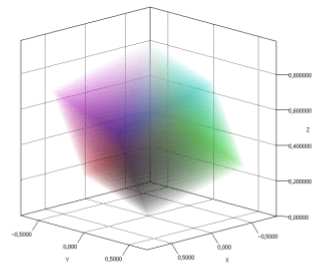
\includegraphics[width=0.5\textwidth]{img/hsi_conversion.png}
\caption{Visualisierung des HSI Farbraums.}
\label{fig:hsi_conversion}
\end{figure}

\subsubsection{Histogramm-Segmentierung}
\label{sec:segmentierung}

Die Samples des Ausgangsbildes werden entlang der Hue-Werte sortiert. Das 1-dimensionale Hue-Histogramm $h=(h_i)_{i = 1 \ldots b}$ mit b-Bins wird gebildet. Gesucht wird nun eine Sequenz $s = (s_i)_{i = 1 \ldots k}$ mit $1 = s_0 < s_1 < \ldots < s_k = b$, welche eine Segmentierung des Histogramms darstellt. Das Intervall $[{s_i}, s_{i+1}]$ wird als Segment bezeichnet. Ziel ist, dass das Histogramm in den Bereichen $[h_{s_i}, \ldots,  h_{s_{i+1}}]$, eine \glqq annähernd unimodale Verteilung aufweist\grqq \citep{acopa}. Abbildung \ref{fig:unimodal} zeigt das Prinzip an verschiedenen Beispielen.

\begin{figure}[h]
\centering
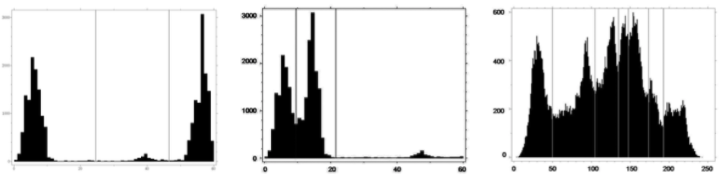
\includegraphics[width=0.48\textwidth]{img/unimodal.png}
\caption{Beispiele der Segmentierung eines Histogramms in unimodale Abschnitte. (Quelle: \citep{acopa})}
\label{fig:unimodal}
\end{figure}

Das Histogramm ist offensichtlich in jedem Segment unimodal, wenn $s$ mit den Minima des Histogramms initialisiert wird. Es wird nun versucht, Elemente aus $s$ zu entfernen, indem für $\forall i = 1 .. k$ überprüft wird, ob $h$ im Intervall $[h_{s_{i-1}}, \ldots,  h_{s_{i+1}}]$ die \glqq unimodale Hypothese\grqq  erfüllt. Anschaulich bedeutet das die Verschmelzung benachbarter Segmente, so dass das neu entstandene Segment nach wie vor \glqq annähernd unimodal ist\grqq. Hierfür stellen die Autoren in einer separaten Veröffentlichung \citep{ftc} einen parameterfreien statistischen Test vor, der $h$ im betrachteten Intervall mit einem Referenz-Histogramm $h^r$ vergleicht. $h^r$ ist in $[h^r_{s_{i-1}}, \ldots,  h^r_{s_{i+1}}]$ zunächst streng monoton wachsend und danach streng monoton fallend und damit in jedem Fall unimodal. Das Referenz-Histogramm wird aus dem Original-Histogramm $h$ durch Anwendung des Grenander-Operators gebildet. Die komplexen Details hierzu sind \citep{acopa, ftc} zu entnehmen. Da der parameterfreie Test verhältnismäßig aufwändig ist, wird in der eigenen Implementierung auf einen simplen T-Test zurückgegriffen. Dieser liefert ebenfalls befriedigende Ergebnisse, ist aber abhängig vom gewählten Signifikanzniveau.

Das Verfahren zur Histogramm-Segmentierung wird in \citep{ftc} als \textbf{Fine-to-Coarse (FTC) Segmentation Algorithm} zusammengefasst. Zunächst wird $s$ mit allen Minima des Histogramms initialisiert. Daraufhin werden so lange benachbarte Segmente durch Überprüfung der unimodalen Hypothese verschmolzen, bis keine Verschmelzung mehr möglich ist. Die Repräsentanten eines Segments werden durch Mittelung der Samples gebildet, die zum jeweiligen Segment gehören. Abbildung \ref{fig:h_segmentation} zeigt dies an einem Beispiel.

\begin{figure}[h]
\centering
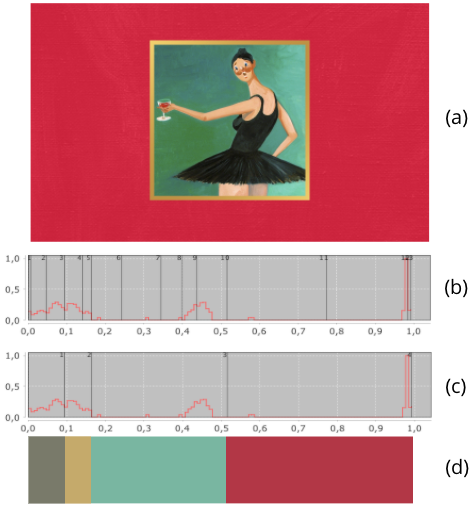
\includegraphics[width=0.48\textwidth]{img/h_segmentation.png}
\caption{Beispiel für eine Segmentierung des Hue-Histogramms. (a) Ausgangsbild, ein Albumcover  von Kanye West. (b) Hue-Histogram (normalisiert), mit allen Minima als initiale Segmentierung. (c) Segmentierung nach Anwendung des FTC Algorithmus. (d) Farbmittelpunkte entsprechend der Samples der jeweiligen Segmente.}
\label{fig:h_segmentation}
\end{figure}

\subsubsection{Bildung der hierarchischen Farbpalette}
\label{sec:hierarchische-farbpalette}

Der ACoPa Algorithmus besteht aus einer hierarchischen Anwendung der Histogram-Segmentierung. Dabei wird zuerst der $h$-, danach der $s$- und abschließend der $i$- Kanal segmentiert. Dabei werden in jedem Schritt die Samples der entstandenen Segmente separiert und die Histogramme der nächsten Ebene getrennt berechnet. Das Ergebnis ist eine hierarchische Farbpalette. Abbildung \ref{fig:palette} zeigt dies am Beispiel der Covers aus Abbildung \ref{fig:h_segmentation}. Auf oberster Ebene (h) wurden die grundsätzlichen Farbtöne des Bildes identifiziert. Auf der zweiten Ebene werden die Farbtöne jeweils in unterschiedliche Sättigungen aufgeteilt, wenn nötig. Auf der dritten Ebene (i) werden von den Sättigungen zusätzlich Helligkeitsabstufungen gebildet.

Die letzte Ebene (i) bildet die Obermenge der Farben $C_s$ für die weitere Verarbeitung. \citet{acopa} empfehlen zusätzlich, die erhaltenen Farben als Startpunkte für den K-Means Algorithmus zu verwenden. Abbildung \ref{fig:palette} (b) zeigt, wie sich die Farben durch K-Means geändert haben. Es ist zu einem späteren Zeitpunkt zu entschieden, welche der beiden Paletten für die weitere Verarbeitung geeigneter ist.

\begin{figure}[h]
\centering
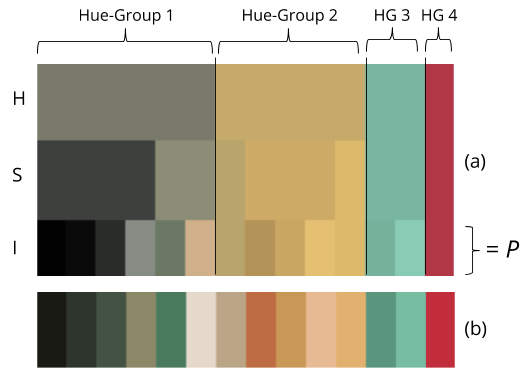
\includegraphics[width=0.48\textwidth]{img/palette.png}
\caption{(a) Hierarchische Farbpalette des Covers aus Abbildung \ref{fig:h_segmentation}. (b) Farbpalette nach Anwendung von K-Means.}
\label{fig:palette}
\end{figure}

\subsection{Vorverarbeitung des Histogramms}
\label{sec:vorverarbeitung}


